% #############################################################################
% This is Appendix Technical Details
% !TEX root = main.tex
% #############################################################################
\chapter{Medical Specifications}
\label{chap:app001}

Appendix~\ref{chap:app001} is a complimentary resource that provides more detailed information, expanding on the topics summarized in Chapter~\ref{chap:chap002}.
It offers in-depth insights into various aspects of the breast cancer domain.
The information provided in Appendix~\ref{chap:app001} further enhances the understanding of the subject matter and provides a comprehensive reference for readers seeking additional background information and medical specifications.

\section{Challenges in Medical Imaging Diagnosis}
\label{sec:app001001}

This section expands on the challenges discussed in Section~\ref{sec:chap002001} of Chapter~\ref{chap:chap002}, providing more detailed information.
The field of medical imaging diagnosis faces significant challenges that affect the efficiency and reliability of the diagnostic process, with one key difficulty being the ever-increasing volume of data to be processed.
Radiologists often struggle to handle this data within reasonable timeframes due to advancements in imaging technologies and the emphasis on early disease detection through screening programs~\cite{HANNA20181709, McKinney2020}.
Addressing this data overload is crucial, necessitating effective solutions capable of handling and analyzing large amounts of medical image data.

In addition to the data volume, the timely analysis of medical images without compromising diagnostic accuracy poses another significant challenge~\cite{10.1145/3399715.3399744, 10.1145/3132272.3134111}.
Radiologists interpret complex images to identify abnormalities and make accurate diagnoses.
However, the manual analysis of extensive image datasets can be time-consuming and subject to human error.
To address these challenges, there has been a growing interest in integrating \ac{AI} techniques into medical imaging practices.
By leveraging AI algorithms and machine learning approaches, medical imaging can potentially improve the efficiency and accuracy of diagnosis~\cite{Lambin2017, pesapane2018artificial, doi:10.1148/radiol.2015151169}.

The emergence of the field of {\it radiomics} (Section~\ref{sec:chap002006} of Chapter~\ref{chap:chap002}) has further propelled the integration of \ac{AI} techniques into medical imaging diagnosis.
Radiomics focuses on extracting quantitative imaging features from medical images on a large scale, aiming to mine valuable information that can assist in diagnosis and treatment planning.
However, to fully unlock the potential of radiomics, extensive data sharing and collaboration are essential for validation and further advancements in the field~\cite{Lambin2017, pesapane2018artificial, doi:10.1148/radiol.2015151169}.
These developments reflect the ongoing efforts to address the challenges faced in medical imaging diagnosis and pave the way for more efficient and accurate diagnostic practices.

\section{Multi-Modal Imaging in Breast Cancer Diagnosis}
\label{sec:app001002}

In the domain of breast cancer diagnosis, the utilization of multi-modal data plays a crucial role in the clinical workflow~\cite{10.1117/1.JBO.22.4.046008}.
While \ac{MG} is the primary imaging modality for breast screening, its effectiveness may be limited in some instances.
For instance, in dense breasts (Figure~\ref{fig:fig005} {\bf B}, {\bf D}), the visibility of lesions is often compromised~\cite{10.1093/jbi/wbaa010}, whereas, in adipose breasts, the visualization of lesions is more precise (Figure~\ref{fig:fig005} {\bf A}, {\bf C}).
Thus, for dense breasts, additional modalities provide valuable information to complement the diagnosis.
Figure~\ref{fig:fig005} {\bf E}, {\bf F} illustrates the use of \ac{US} and \ac{DCE-MRI} modalities, where the lesions can be easily identified.
Among various imaging characteristics, the ultimate objective is to classify tumors into benign or worrisome categories based on their severity~\cite{SHAN2016980}.

%%%%%%%%%%%%%%%%%%%%%%%%%%%%%%%%%%%%%%%%%%%%%%%%%%
\begin{figure}[htbp]
\centering
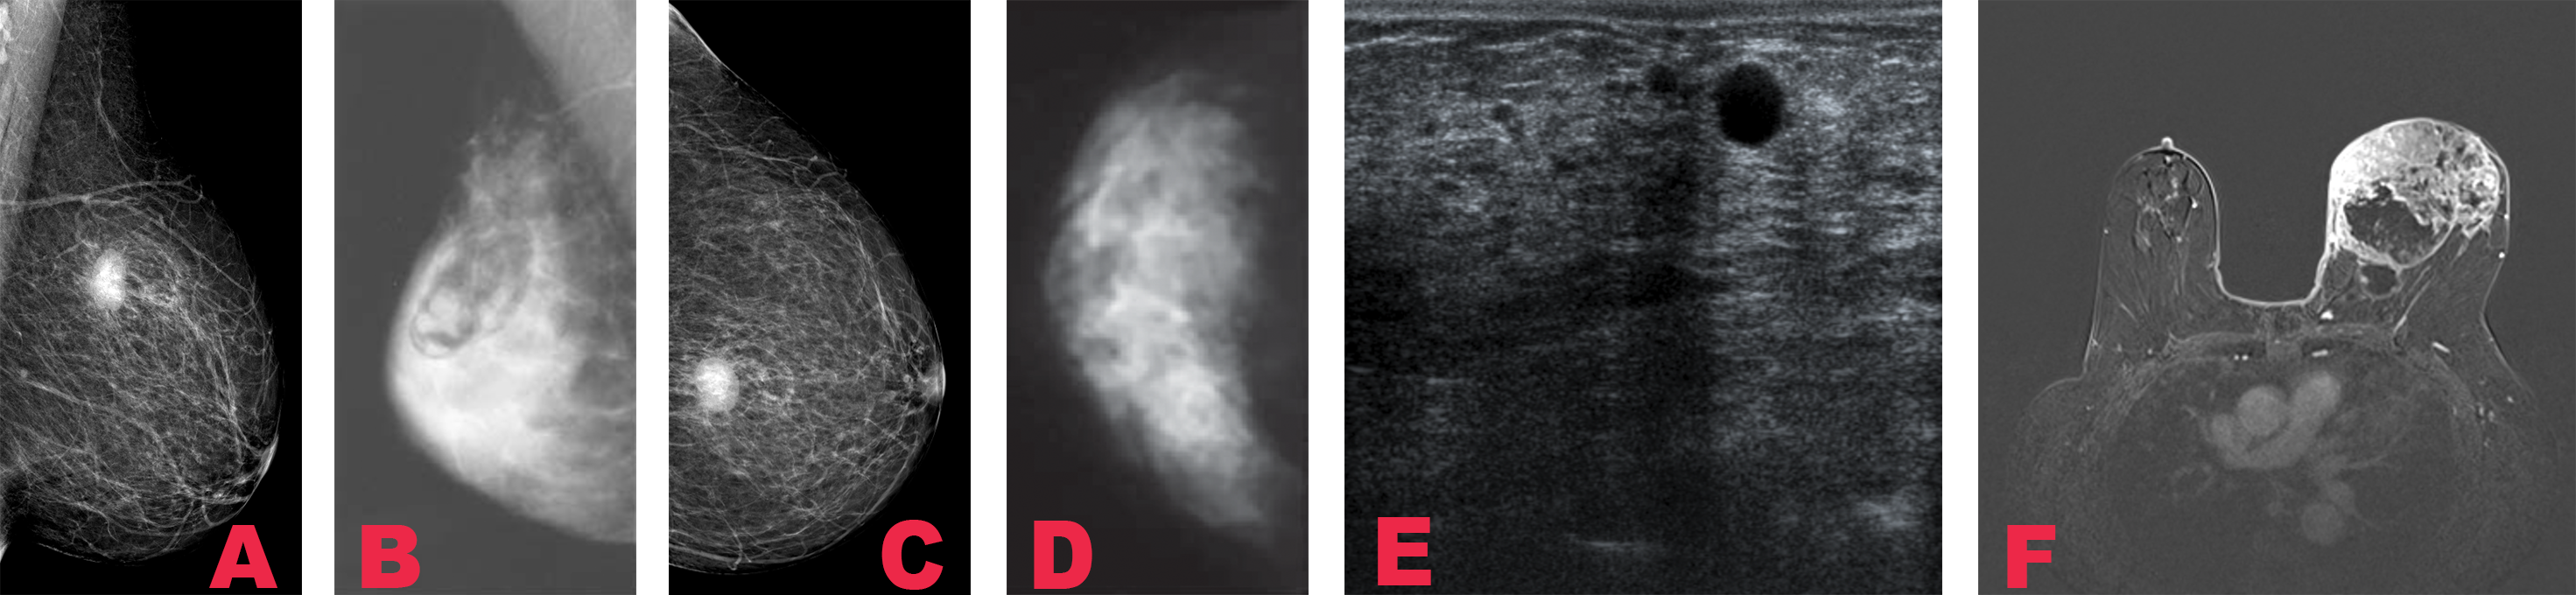
\includegraphics[width=\columnwidth]{images/fig005}
\caption{Illustration of the current clinical setup. Adipose breast in MG, where the lesions are easily viewed (A, C). Dense breast where it is not possible to view the lesions (B, D). In the latter scenario, the radiologists resort to other image modalities, such as US (E) and DCE-MRI (F), to complement the information that is missing in (B, D).}
\label{fig:fig005}
\end{figure}
%%%%%%%%%%%%%%%%%%%%%%%%%%%%%%%%%%%%%%%%%%%%%%%%%%

In the current clinical setup, integrating different imaging modalities is employed to overcome the limitations of mammograms.
Adipose breasts (Figure~\ref{fig:fig005} {\bf A}, {\bf C}) benefit from the visibility provided by \ac{MG} alone.
However, in cases of dense breasts (Figure~\ref{fig:fig005} {\bf B}, {\bf D}), where \ac{MG} alone may not be sufficient, additional modalities such as ultrasound and \ac{DCE-MRI} are used to complement the missing information (Figure~\ref{fig:fig005} {\bf E}, {\bf F}).
These complementary modalities improve the accuracy and reliability of breast cancer diagnosis, allowing radiologists to make more informed decisions regarding the nature and severity of detected tumors.
Integrating multi-modal imaging techniques in the breast cancer domain showcases the importance of combining different modalities to enhance diagnostic capabilities and improve patient outcomes.
This section expands upon the summary provided in Section~\ref{sec:chap002002} of Chapter~\ref{chap:chap002}.

\section{Breast Lesion Classification}
\label{sec:app001003}

Clinical guidelines advise regular image screenings as part of assessing the risk of breast cancer~\cite{MIAO201817}.
However, accurately interpreting and classifying the findings from breast imaging can be challenging due to variations in radiologists' descriptions and interpretations.
To address this issue, the \acf{ACR} developed the \acf{BI-RADS}~\cite{d2018breast}.
The \ac{BI-RADS} provides a standardized lexicon and a classification system with six categories\footnotemark[15] to evaluate the likelihood of malignancy.
It enhances precision and uniformity in breast cancer diagnoses by establishing a standardized framework for characterizing imaging findings and reducing ambiguity.

%%%%%%%%%%%%%%%%%%%%%%%%%%%%%%%%%%%%%%%%%%%%%%%%%%%
\footnotetext[15]{\acs{BI-RADS}: stands for \acf{BI-RADS}, which is a scale for putting the findings from breast cancer diagnosis into a few well-defined categories. The scale ranges from 0 to 6 (see more at \hyperlink{https://breast-cancer.ca/bi-rads/}{breast-cancer.ca/bi-rads}). However, for the simplicity of the study, we just considered a 1 to 5 scale range. Radiologists can only score a 6 after a biopsy, and a 0 means that the study needs additional imaging.}
%%%%%%%%%%%%%%%%%%%%%%%%%%%%%%%%%%%%%%%%%%%%%%%%%%%

Radiologists use the \ac{BI-RADS} categories to assess and communicate the level of suspicion for malignancy associated with various imaging features (Section~\ref{sec:chap002004} of Chapter~\ref{chap:chap002}), such as masses, calcifications, architectural distortion, and asymmetry.
This system enables radiologists to convey their observations effectively, ensuring that critical information regarding lesion characteristics and potential malignancy is conveyed consistently.
The \ac{BI-RADS} categories help guide subsequent management decisions, such as the need for further imaging, biopsy, or follow-up, based on the level of suspicion for malignancy indicated by the classification.

The \ac{BI-RADS} classification system allows radiologists to communicate the breast imaging results clearly and consistently.
It provides a standardized framework for describing imaging findings (Figure~\ref{fig:fig020}), assigning a final assessment category, and providing specific recommendations for further evaluation or follow-up.
The categories range from 0 to 6, with 0 indicating the need for additional imaging and 6 indicating a known malignancy confirmed by biopsy.
Using the \ac{BI-RADS} system, radiologists can enhance communication with referring physicians and ensure appropriate management of patients with breast lesions.

%%%%%%%%%%%%%%%%%%%%%%%%%%%%%%%%%%%%%%%%%%%%%%%%%%
\begin{figure}[ht]
\centering
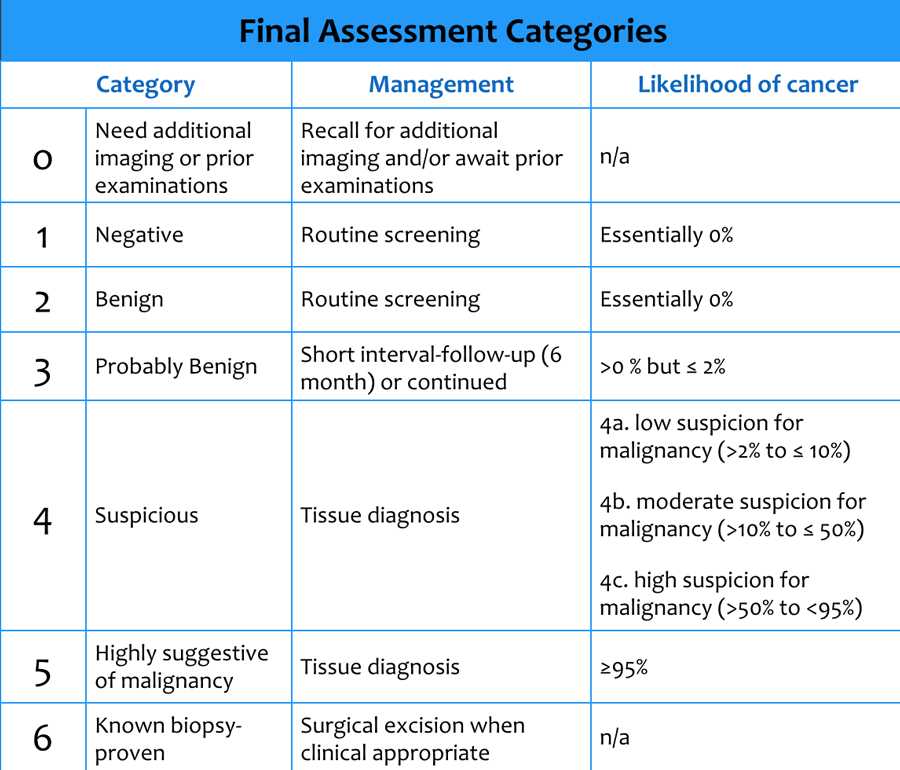
\includegraphics[width=\columnwidth]{images/fig020}
\caption{The BI-RADS enables radiologists to communicate results clearly and consistently, with a final assessment and specific recommendations. Image from \protect\href{https://radiologyassistant.nl/breast/bi-rads/bi-rads-for-mammography-and-ultrasound-2013}{radiologyassistant.nl} in June 2023.}
\label{fig:fig020}
\end{figure}
%%%%%%%%%%%%%%%%%%%%%%%%%%%%%%%%%%%%%%%%%%%%%%%%%%

In this thesis, several \acp{DNN} are trained to classify breast lesions according to standardized \ac{BI-RADS} categories.
The trained \acp{DNN} utilizes \ac{ML} techniques and analyzes large labeled image datasets to recognize intricate patterns and extract distinctive features indicative of different breast lesion categories.
The main objective of this research is to develop a reliable and accurate intelligent agent that assists radiologists in classifying breast lesions, thereby improving diagnostic accuracy and patient outcomes.
Specifically, this intelligent agent functions as a valuable autonomous second reader, leveraging its computational capabilities to analyze complex imaging data and provide additional insights to complement the expertise of radiologists.
This section highlights the crucial attributes of breast lesion classification discussed in Section~\ref{sec:chap002003} of Chapter~\ref{chap:chap002}, where the \ac{BI-RADS} nomenclature is introduced.
Appendix~\ref{chap:app004} provides comprehensive details on the number of screened patients and images used to train and validate the initial \ac{DL} models, as described in Section~\ref{sec:app004003002}.

\section{Significance of Lesion Typification}
\label{sec:app001004}

Addressing the critical challenge of lesion typification, this thesis emphasizes the pivotal role it plays in breast cancer diagnosis.
While lesion typification was introduced in Section~\ref{sec:chap002004} of Chapter~\ref{chap:chap002}, this section elaborates further.
The primary objective is to underscore the importance of lesion typification, with a specific focus on masses (Section~\ref{sec:chap002004001}) and microcalcifications (Section~\ref{sec:chap002004002}).
These lesions offer invaluable information that informs the \ac{AI} algorithms developed in Chapter~\ref{chap:chap005} and Chapter~\ref{chap:chap006}, facilitating accurate breast cancer diagnosis.
A comprehensive understanding of different mass shapes, microcalcification patterns, and sizes is essential for effectively classifying the severity of breast lesions~\cite{8611096, 9231684}, as these factors significantly impact algorithm performance.
By shedding light on the significance of lesion typification, this section unveils the critical factors contributing to improved diagnostic accuracy and enhanced patient outcomes in breast cancer.

\subsection{Mass Typification and Margins}
\label{sec:app001004001}

This section provides a deeper exploration of the complexities involved in accurately classifying breast masses and reinforces their importance in breast cancer diagnosis.
It expands on the information summarized in Section~\ref{sec:chap002004001} of Chapter~\ref{chap:chap002}, shedding light on the specific characteristics of different mass shapes and the significance of margin assessment in determining the nature of the mass.
Accurate classification of breast masses is vital in diagnosing and planning treatment for breast cancer patients, as distinguishing between benign and malignant masses is a critical initial step in determining the appropriate action.
Visual representations of different mass shapes encountered in breast imaging, as depicted in Figure~\ref{fig:fig021}, provide valuable insights for radiologists and \ac{AI} algorithms.

%%%%%%%%%%%%%%%%%%%%%%%%%%%%%%%%%%%%%%%%%%%%%%%%%%
\begin{figure}[htpb]
\centering
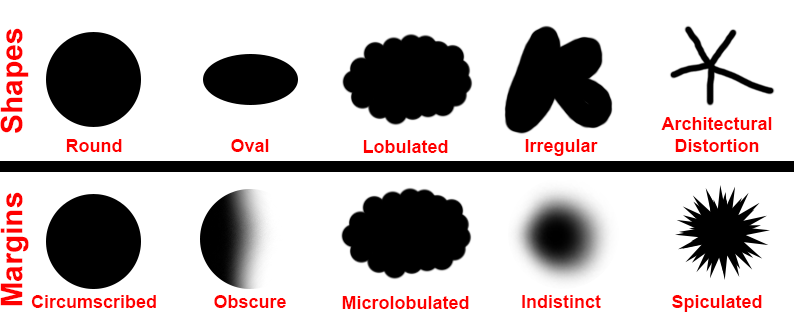
\includegraphics[width=\columnwidth]{images/fig021}
\caption{[DOI: \href{https://doi.org/10.13140/RG.2.2.33693.26086}{10.13140/RG.2.2.33693.26086}] Lesion Types - First line is showing the type of {\bf Shapes}: {\bf Round}, {\bf Oval}, {\bf Lobulated}, {\bf Irregular}, and {\bf Architectural Distortion}. The second line shows the type of {\bf Margins} of the lesion: {\bf Circumcribed}, {\bf Obscure}, {\bf Microlobulated}, {\bf Indistinct}, and {\bf Spiculated}.}
\label{fig:fig021}
\end{figure}
%%%%%%%%%%%%%%%%%%%%%%%%%%%%%%%%%%%%%%%%%%%%%%%%%%

Benign masses often exhibit round, oval, or lobulated shapes with well-defined boundaries and regular contours.
These masses are typically non-threatening and may represent benign conditions such as cysts or fibroadenomas.
Conversely, lobulated, irregular, and architectural distortion shapes are frequently associated with malignant masses.
These shapes demonstrate complex and asymmetrical characteristics, suggesting the presence of cancerous cells within the mass.

Analyzing the shape of breast masses allows radiologists and \ac{AI} algorithms to gather initial clues regarding the potential nature of the lesion.
However, it is essential to emphasize that shape alone cannot diagnose definitively.
A comprehensive assessment requires the consideration of additional imaging features and clinical information to establish an accurate diagnosis and determine the most suitable management strategy for each patient.

When assessing breast lesions, it is crucial to consider the characteristics of the margins. Five types of margins can provide valuable information for diagnosis.
A circumscribed margin typically indicates a benign lesion, suggesting that it is well-defined and has a clear boundary.
On the other hand, the presence of microlobulated, indistinct, or spiculated margins raises suspicion, with spiculated margins being the most concerning.
An obscured margin is observed when part of the margin is concealed by fibroglandular tissue.
If a patient's case shows an obscured margin, performing an \ac{US} examination (Figure~\ref{fig:fig018}) is recommended to evaluate the lesion further and gather additional information.
Ultimately, assessing the lesion's margins contributes to accurate diagnosis and clinical decisions.

\subsection{Role of Microcalcification Patterns}
\label{sec:app001004002}

The role of microcalcification patterns in breast cancer diagnosis is of significant importance.
In this section, we provide a detailed exploration of the typification of microcalcifications, encompassing five distinct types as identified in the literature.
These patterns, ranging from less malignant to more malignant, are visually represented in Figure~\ref{fig:fig022}.
It is essential to note that this section expands upon the summarization of microcalcification patterns discussed in Section~\ref{sec:chap002004002} of Chapter~\ref{chap:chap002}, providing further insights into their significance and implications for breast cancer diagnosis.
Through a thorough exploration of these patterns, we aim to deepen our understanding of their role in the identification and characterization of potential malignancies in breast imaging.

In breast imaging, the identification and interpretation of microcalcification patterns play a crucial role in the detection and characterization of breast abnormalities.
The first pattern, known as the diffuse pattern (letter {\bf a} of Figure~\ref{fig:fig022}), describes the random dispersion of microcalcifications throughout the breast tissue.
This pattern is often associated with benign conditions, such as fibrocystic changes, where the microcalcifications are evenly distributed without a specific clustering pattern.
However, in some cases, diffuse microcalcifications may also indicate early-stage malignancies, such as \ac{DCIS}, requiring further evaluation~\cite{10.1093/jnci/djaa080}.

%%%%%%%%%%%%%%%%%%%%%%%%%%%%%%%%%%%%%%%%%%%%%%%%%%
\begin{figure}[ht]
\centering
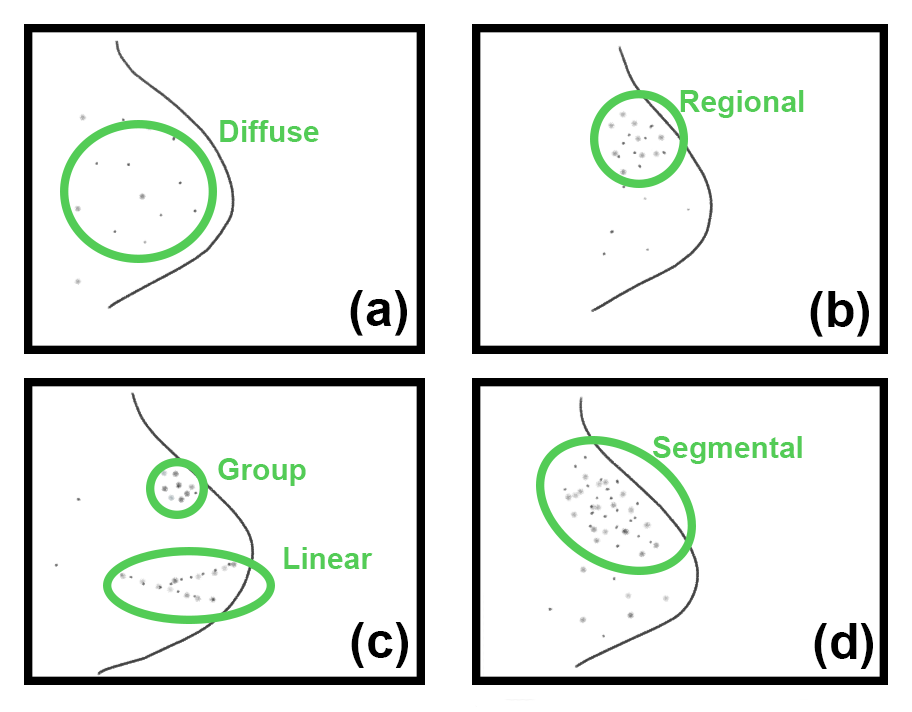
\includegraphics[width=\columnwidth]{images/fig022}
\caption{[DOI: \href{https://doi.org/10.13140/RG.2.2.26667.80164}{10.13140/RG.2.2.26667.80164}] Calcification Types - The {\bf Diffuse} is when the microcalcifications are ``randomly'' spread across the image. The {\bf Regional} is when the microcalcifications are close to each other, forming a sort of ``circle''. The {\bf Group} is a small area with few microcalcifications. The {\bf Linear} is when the microcalcifications form ``lines''. The {\bf Segmental} is similar to the {\bf Regional} but approaches a more oval shape instead of a circular.}
\label{fig:fig022}
\end{figure}
%%%%%%%%%%%%%%%%%%%%%%%%%%%%%%%%%%%%%%%%%%%%%%%%%%

The regional pattern (letter {\bf b} of Figure~\ref{fig:fig022}) involves the presence of multiple microcalcifications occupying a localized region of the breast, typically spanning over two centimeters in diameter.
This pattern can raise suspicion for malignancy, as it may indicate the presence of a growing tumor or an area of proliferative breast disease.
Further assessment and correlation with other imaging findings are necessary to determine the likelihood of malignancy and guide subsequent management decisions.

The group pattern (letter {\bf c} of Figure~\ref{fig:fig022}) refers to a small cluster of microcalcifications within a limited area of the breast.
This pattern can vary in size and shape, and while it can be seen in both benign and malignant cases, it often requires careful evaluation to assess its significance.
Additional imaging views and comparisons with prior examinations are commonly performed to evaluate the stability and growth of the microcalcification cluster, aiding in determining its likelihood of malignancy.
Radiologists play a critical role in interpreting these findings and ensuring optimal outcomes.

The linear pattern (letter {\bf c} of Figure~\ref{fig:fig022}) is characterized by microcalcifications arranged in a linear configuration.
This pattern is suggestive of the deposition of calcifications within a duct, often associated with intraductal pathologies.
While linear microcalcifications can be seen in benign and malignant cases, their distribution, morphology, and associated imaging features are carefully evaluated to determine the level of concern and guide further management.

Lastly, the segmental pattern (letter {\bf d} of Figure~\ref{fig:fig022}) involves the presence of microcalcifications in a duct or multiple ducts, including their branches.
This pattern typically indicates a more extensive distribution of microcalcifications within a specific segment of the breast.
Segmental microcalcifications can be associated with various breast conditions, including benign and malignant processes.
Further evaluation, correlation with clinical findings, and consideration of additional imaging modalities are often necessary to establish an accurate diagnosis and guide patient management.

In breast cancer diagnosis, typifying microcalcifications based on patterns is crucial in radiological interpretation.
Each pattern carries specific associations and implications, but a comprehensive evaluation is necessary for the final assessment.
This includes considering additional imaging features, clinical information, and, in some cases, histopathological analysis.
The impact of multimodality requirements~\cite{https://doi.org/10.1002/cncr.32910} on the clinical workflow (Figure~\ref{fig:fig018}), as \ac{MG} alone, may not provide a complete dataset for accurate diagnosis from clinicians and \ac{AI} algorithms~\cite{DANA2020541}.
More details on the current imaging workflow and the significance of multimodal data availability can be found in Section~\ref{sec:chap002005} of Chapter~\ref{chap:chap002}.

\section{Radiological Workflow}
\label{sec:app001005}

This section expands upon the summarization provided in Section~\ref{sec:chap002005} of Chapter~\ref{chap:chap002}, offering more insights into the radiological workflow.
The main \ac{RRR} workflow (Figure~\ref{fig:fig018}) can be defined as a three-stage process:
(1) {\it examination};
(2) {\it diagnosis}; and
(3) {\it report}.
The {\it examination} stage (Section~\ref{sec:app001005001}) refers to the time spent on the examination and processing of the patient records ({\it e.g.}, demographics, clinical records, or past medical images).
For instance, the radiologist receives this information from the hospital and radiology information systems~\cite{islam2018recent}.
The second stage, {\it i.e.}, {\it diagnosis} (Section~\ref{sec:app001005002}), corresponds to the time that the radiologist spends on the interpretation and diagnosis of the patient exams.
In this phase, the radiologist interacts with a \ac{PACS} retrieving the {\it modality working list} from a radiology information system~\cite{DIROBERTO2016950} of the hospital.
Finally, in the last stage, {\it i.e.}, {\it report} (Section~\ref{sec:app001005003}), it refers to the time spent on reporting her/his conclusions after the patient's medical images analysis.
These insights enhance our understanding of the intricate radiological workflow, particularly in the collaboration between \ac{HCI} and \ac{AI} communities for assisting radiologists during a breast cancer diagnosis.
The meticulous work of both communities and healthcare practitioners is vital for timely and impactful breast cancer detection, improving patient outcomes.

%%%%%%%%%%%%%%%%%%%%%%%%%%%%%%%%%%%%%%%%%%%%%%%%%%%
\begin{figure}[ht]
\centering
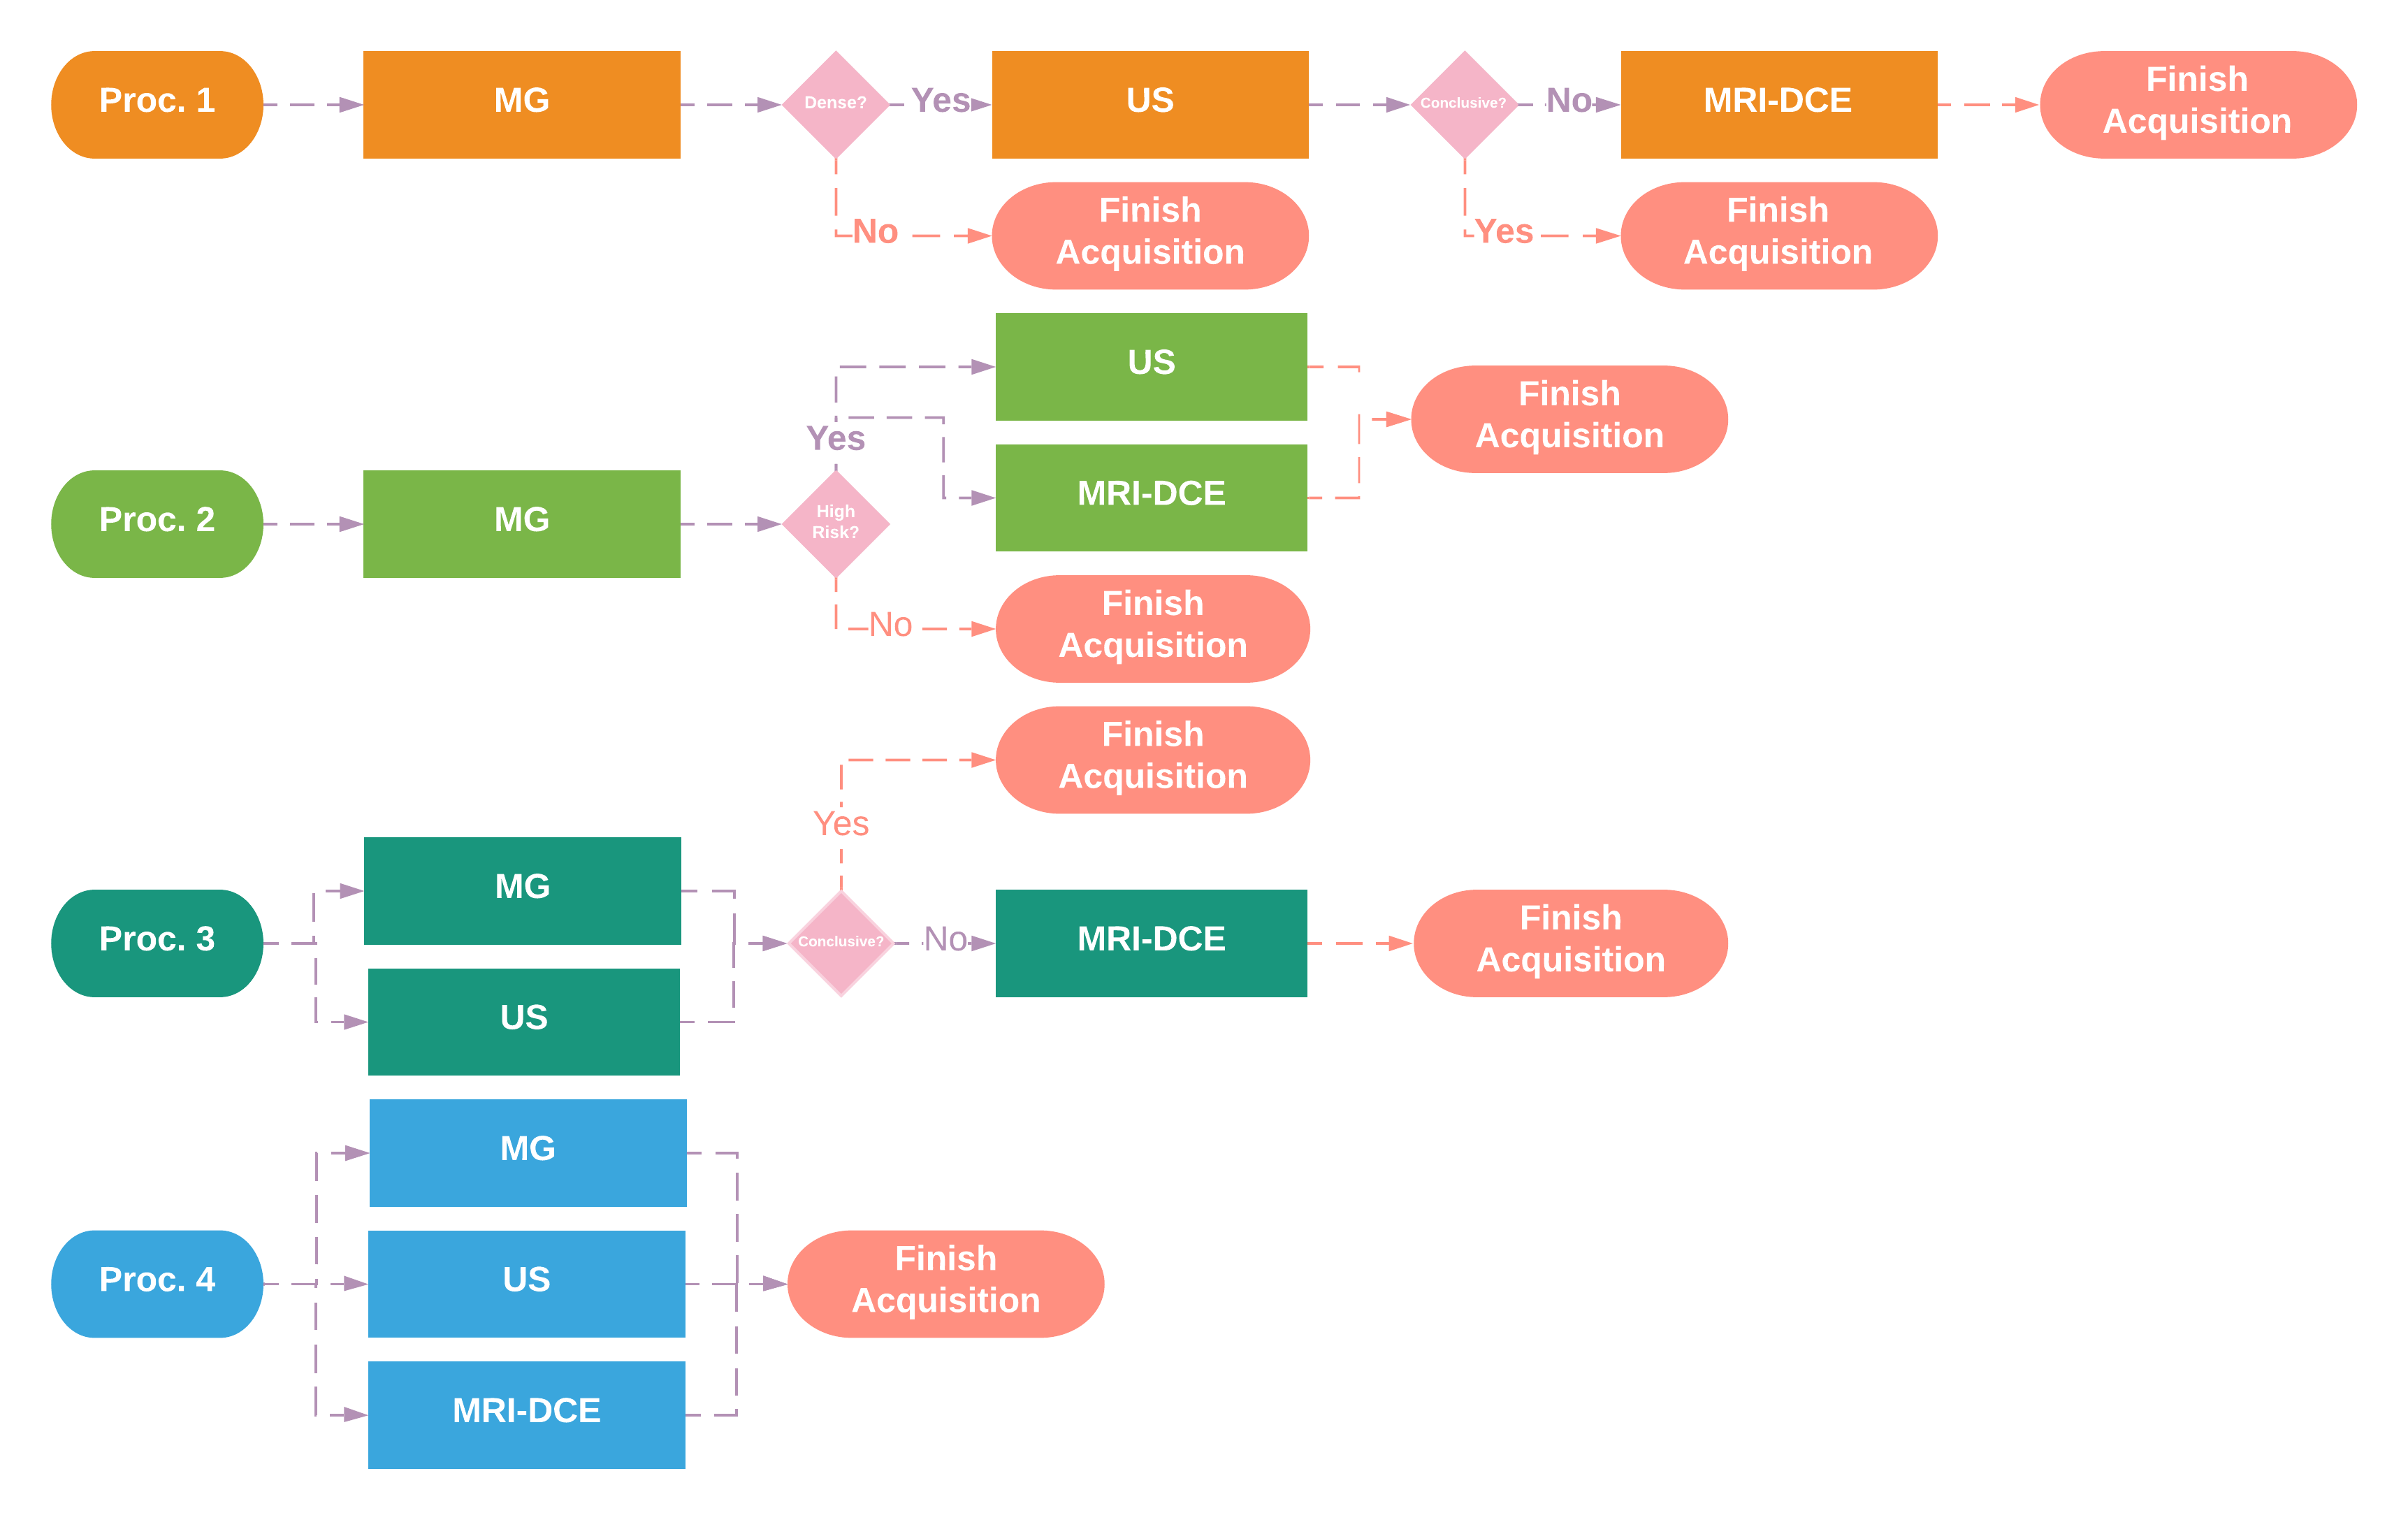
\includegraphics[width=\columnwidth]{images/fig018}
\caption{Workflow of the radiology reading room is commonly adopted in clinical institutions using several image acquisition strategies. Screening modalities ({\it e.g.}, US, MRI, etc.) constitute important complementary information for a reliable diagnosis.}
\label{fig:fig018}
\end{figure}
%%%%%%%%%%%%%%%%%%%%%%%%%%%%%%%%%%%%%%%%%%%%%%%%%%%

In all the above stages, images play a crucial role in the diagnosis and management of breast cancer.
They serve different purposes and provide valuable information for accurate assessments.
The collaboration among the nine clinical institutions highlighted in Chapter~\ref{chap:chap005} further strengthens the understanding and implementation of these workflow stages.
In the following sections, we delve into each stage, examining their significance and impact in detail.

\subsection{Image Examination}
\label{sec:app001005001}

In the initial stage of the radiological workflow, known as the {\it examination} stage~\cite{8621479}, the radiologist conducts a thorough review of the patient's medical imaging, correlating it with other relevant exams and records to obtain a comprehensive understanding of the clinical context.
During this stage, the radiologist relies on various sources of information to enhance the accuracy and reliability of the examination process~\cite{islam2018recent, DIROBERTO2016950}.
These may include integrated systems that provide access to a centralized database of patient information, facilitating the retrieval of past exams, reports, and notes from the referring physician.
Furthermore, the radiologist may seek second opinions from other healthcare professionals to gain additional insights into the patient's medical history and optimize the diagnostic process~\cite{GIBSON2018113}.

The examination stage is a critical component of the radiological workflow, as it establishes the foundation for the subsequent stages of diagnosis and reporting.
By carefully analyzing the available information and integrating it with the medical images, the radiologist gains valuable insights into the patient's condition, enabling them to make informed decisions and recommendations for further evaluation and treatment.
This comprehensive examination ensures that all relevant clinical data are considered, contributing to accurate and personalized breast cancer diagnosis.

\subsection{Patient Diagnosis}
\label{sec:app001005002}

Regarding the {\it diagnosis} stage~\cite{https://doi.org/10.1002/cncr.32872}, this is the most crucial from this document's perspective, as it significantly influences the treatment choice.
The {\it diagnosis} stage involves image classification (Section~\ref{sec:chap002003}) using the \ac{BI-RADS} scale, and clinicians were observed accessing multiple medical images during this process.
Several studies (Chapter~\ref{chap:chap005}) were conducted to understand clinicians' needs during decision-making and their interactions with intelligent agents.

At this stage, each 2D medical imaging modality takes approximately 120 seconds to analyze, meaning clinicians spend around two minutes interpreting each imaging type~\cite{jiang2018interpretation}.
However, in most cases, each patient requires the analysis of more than six 2D images and several other 3D volume sequences\footnotemark[16] (e.g., MRI volumes can have over 100 frames per sequence).
As a result, a complete diagnosis in an actual situation (i.e., reviewing all modalities, clinical records, and reporting the patient's case) can take more than an hour of the clinician's time~\cite{Forsberg2017}, making this task cumbersome and prone to errors.

%%%%%%%%%%%%%%%%%%%%%%%%%%%%%%%%%%%%%%%%%%%%%%%%%%%
\footnotetext[16]{The \ac{MRI} volumes comprises different types of sequences, concretely, T1, T2, T2 Fat Sat, Diffusion, \ac{DCE}-\ac{MRI}, \ac{DCE}-\ac{MRI} with subtraction in five time instants. The sensitivity of \ac{MRI} makes it an excellent tool in specific clinical situations. Situations such as the screening of patients at high risk, and evaluation of the extent of disease in patients with a new diagnosis. Compared to \ac{MG} and \ac{US}, \ac{MRI} provides higher sensitivity; however, its specificity is variable. Moreover, \ac{MRI} data analysis is time-consuming and depends on reader expertise.}
%%%%%%%%%%%%%%%%%%%%%%%%%%%%%%%%%%%%%%%%%%%%%%%%%%%

Observations (Section~\ref{sec:chap005003002} of Chapter~\ref{chap:chap005}) have revealed that the overwhelming volume of medical images and the limited time for each patient's diagnosis can contribute to clinicians disengaging from reviewing all medical images.
The complexity and time constraints of the diagnostic process may cause clinicians to focus on critical findings or prioritize specific images, potentially overlooking subtle but clinically significant pathologies.
Various factors, such as fatigue, workload, and the need for efficient decision-making, can influence this selective attention.

The consequences of disengagement or the disregard of specific pathologies in medical images (Section~\ref{sec:chap002004} of Chapter~\ref{chap:chap002}) can be detrimental to accurate diagnosis and patient care.
Even minor abnormalities or early signs of disease can hold crucial diagnostic information that may impact treatment decisions and patient outcomes~\cite{doi:10.1148/radiol.2020192534}.
Therefore, efforts are being made to develop advanced technologies and intelligent systems that can assist radiologists in detecting and interpreting relevant findings in medical images, helping to mitigate the risk of human errors and enhance diagnostic accuracy.

\subsection{Final Report}
\label{sec:app001005003}

The {\it final report} stage, which occurs after the patient classification, is crucial in improving the patient's clinical records and determining the prognosis.
During this stage, the clinician thoroughly examines the patient's records and carefully analyzes each medical image to generate a comprehensive report.
To streamline this process, many clinicians utilize dictating systems that allow them to record their findings and impressions verbally.
These recorded reports are then transcribed into written documents, which are later reviewed and signed by the clinicians to finalize the diagnostic report.

The final report is a critical communication tool, capturing the radiologist's interpretations, assessments, and recommendations.
It provides essential information to other healthcare professionals involved in the patient's care, such as referring physicians and oncologists, guiding them in developing appropriate treatment plans.
The final report documents the radiologist's findings, ensuring continuity of care, facilitating collaboration, and enabling informed decision-making.
Furthermore, these reports become part of the patient's medical records, serving as a valuable resource for future reference and comparison in subsequent examinations and follow-up visits.

\subsection{Summarizing Clinical Procedures}
\label{sec:app001005004}

As previously discussed (Section~\ref{sec:app001004}), using images to display breast lesions vary widely across medical imaging modalities (\ac{MG}, \ac{US} and \ac{DCE}-\ac{MRI}, being the two latter modalities crucial for dense breasts).
Multimodality (Section~\ref{sec:app001002}) is responsible for increasing the cognitive load of radiologists and increasing detection rates, but also reducing \acp{FP} and \acp{FN}.
In this section, we define and describe the main clinical procedures, while the topic was first introduced in Section~\ref{sec:chap002005} of Chapter~\ref{chap:chap002}.

\vspace{1.50mm}

\noindent
The main clinical procedures (Figure~\ref{fig:fig018}) of the \ac{RRR} workflow usually comprises four different paths that correspond to different observed image acquisition procedures:

\vspace{0.05mm}

%%%%%%%%%%%%%%%%%%%%%%%%%%%%%%%%%%%%%%%%%%%%%%%%%%%
\begin{enumerate}
\item \textbf{Procedure 1} starts with the acquisition of \ac{MG}, then, if the breast is dense, the \ac{US} modality is acquired. Finally, if the \ac{MG} and \ac{US} are not conclusive, the \ac{DCE}-\ac{MRI} is acquired, otherwise the process is concluded;
\item \textbf{Procedure 2} starts with the acquisition of \ac{MG}, then if the clinician detects a high risk of cancer from the image patterns and/or patient records, both \ac{US} and \ac{DCE}-\ac{MRI} are acquired; otherwise the process is concluded;
\item \textbf{Procedure 3} \ac{MG} and \ac{US} are acquired simultaneously, if the {\it exam} is still not conclusive, the \ac{DCE}-\ac{MRI} is acquired;
\item \textbf{Procedure 4} all three modalities (\ac{MG}, \ac{US} and \ac{DCE}-\ac{MRI}) are acquired simultaneously.
\end{enumerate}
%%%%%%%%%%%%%%%%%%%%%%%%%%%%%%%%%%%%%%%%%%%%%%%%%%%

From the interviews and observations (Section~\ref{sec:chap005003002} of Chapter~\ref{chap:chap005}), it was found that radiologists access medical images in two main scenarios:
i) imaging perception process, namely to detect patterns of lesions;
and ii) finding relationships between past lesion patterns and possible future diagnosis.
Given the time constraints and the amount of information available, clinicians often do not observe all the images with the necessary detail.
From these observations (Section~\ref{sec:chap005003002}), it was concluded that they start by analyzing the patient's clinical history (when available).
Ultimately, the clinical history provides the necessary knowledge to guide the analysis of the current state and the basis of {\it radiomics}.
In the next section, the document will introduce the basics and definitions of extracting information from medical images, such as the {\it radiomics} topic introduced in Section~\ref{sec:chap002006} of Chapter~\ref{chap:chap002}.

\section{Extracting Information from Medical Images}
\label{sec:app001006}

The section expands on the summarization provided in Section~\ref{sec:chap002006} of Chapter~\ref{chap:chap002}, offering a deeper understanding of the topic and its relevance in improving clinical decision-making.
The topic of {\it radiomics} is a growing field that aims at extracting and mining information from medical images.
Specifically, the goal is to develop computerized support systems to improve clinical decision-making.
Among the clinical tasks, breast cancer diagnosis is one of the main areas where {\it radiomics} is growing.

\ac{CADx} systems can be developed to improve the diagnostic pipeline through automatic tumor malignancy assessment and reduction of negative diagnostic rates.
Through these \ac{CADx} systems, the application of {\it radiomics} to breast cancer may result in the acquisition of essential information for feature modelling~\cite{10.1007/978-3-030-59716-0_71}.
Similar to what we are doing in this thesis, introducing intelligent agents for feature modeling in \ac{CADx} systems will result in better breast cancer characterization.
Accurate communication of intelligent agents will have the potential to improve diagnostic performance by a decrease in sensitivity and specificity of the medical errors~\cite{doi:10.1148/radiol.2020192039}.
For breast tumor classification (Section~\ref{sec:chap002003} of Chapter~\ref{chap:chap002}), this section also needs to address the {\it radiomics} pipeline (Figure~\ref{fig:fig023}) that will be employed to extract imaging features from tumor images.

%%%%%%%%%%%%%%%%%%%%%%%%%%%%%%%%%%%%%%%%%%%%%%%%%%%
\begin{figure}[htbp]
\centering
\includegraphics[width=\columnwidth]{images/fig023}
\caption{Breast tumors are analyzed through this pipeline, where {\it radiomics}, paired with AI, ML, and DL techniques, is of chief importance, to recognize image-based patterns and perform the diagnostic classification based on quantitative imaging features.}
\label{fig:fig023}
\end{figure}
%%%%%%%%%%%%%%%%%%%%%%%%%%%%%%%%%%%%%%%%%%%%%%%%%%%

Several techniques are employed to analyze (letter {\bf a} of Figure~\ref{fig:fig023}) imaging features.
From tumor images, automatic segmentation can delineate the lesion contours (Figure~\ref{fig:fig021}), as well as extract texture, shape, and margin (Section~\ref{sec:chap002004001}).
With these feature extraction (letter {\bf c} of Figure~\ref{fig:fig023}), the descriptors of {\it radiomics} can characterize, {\it i.e.}, detect (letter {\bf b} of Figure~\ref{fig:fig023}) and classify (letter {\bf d} of Figure~\ref{fig:fig023}), the lesion.
Further, it will be possible to compare the autonomous with the clinician characterization.

In this thesis, several {\it radiomics} are extracting quantitative features to train various classifiers.
The aim is to extract the quantified characteristics for an available and curated dataset (Chapter~\ref{chap:chap004}) of breast images with the aid of automated algorithms and respective intelligent agents.
There have been numerous pipelines and methods developed, although the lack of standardization in medical image processing makes it difficult to consume different formats.
Thus, in Section~\ref{sec:chap002007}, this challenge is addressed.

Despite the success of \ac{DL}, and even though different studies have shown that {\it radiomics} ({\it i.e.}, \ac{AI}-assisted methods for medical image analysis) can reduce human error and improve outcomes, their adoption by the medical community has been slow.
One of the main reasons is the inability of these systems to provide relevant medical information or to capture the nuances of the human mind~\cite{kohli2018cad, 10.1145/2858036.2858373}, making them untrustworthy and preventing their clinical acceptance.
In particular, \ac{DL}-based methods have been frequently viewed as `black box' approaches~\cite{litjens2017survey}.
Therefore, \ac{HCI} plays an essential role in creating user-friendly interactive systems for \ac{AI}-assisted medical image analysis~\cite{10.1145/3132272.3134111}.

\section{Standardization in Medical Imaging}
\label{sec:app001007}

In this section, we expand upon the details summarized in Section~\ref{sec:chap002007} of Chapter~\ref{chap:chap002}, providing a deeper exploration of the standardization aspects in medical imaging.
The \ac{DICOM} format\footnotemark[17] plays a crucial role in the storage of medical images, serving as a standard in the field of medicine~\cite{Trivedi2019}.
It offers extensive support for various types of medical information, including exam images and structured reports.
Additionally, one of its advantages is the ability to convert known file formats, such as \ac{JPEG} and \ac{MPEG}, ensuring compatibility and interoperability.
This section explores the significance of standardized medical imaging and its implications for medical systems.

%%%%%%%%%%%%%%%%%%%%%%%%%%%%%%%%%%%%%%%%%%%%%%%%%%%
\footnotetext[17]{For more details, follow the ``\href{https://medium.com/oppr/using-cornerstonejs-and-orthanc-to-support-deep-learning-projects-c9675819c33a}{Using CornerstoneJS and Orthanc to Support Deep Learning Projects}'' article (\href{https://link.medium.com/LNZ5glN1c4}{link.medium.com/LNZ5glN1c4}). Accessed on 26th of June 2023. It requires an internet connection.}
%%%%%%%%%%%%%%%%%%%%%%%%%%%%%%%%%%%%%%%%%%%%%%%%%%%

A \ac{DICOM} file encodes medical information as a dataset, organized in the form of an associative array (Figure~\ref{fig:fig025}).
This dataset structure allows for a hierarchical arrangement of data, resembling the format of a \ac{JSON} file (Section~\ref{sec:app004009} of Appendix~\ref{chap:app004}).
Moreover, each value within the dataset can be a list of datasets, further contributing to the hierarchical nature of the data structure.
This flexibility enables the representation of complex medical information with multiple levels of a {\it framework} (Appendix~\ref{chap:app008}), facilitating the storage and retrieval of relevant data.

%%%%%%%%%%%%%%%%%%%%%%%%%%%%%%%%%%%%%%%%%%%%%%%%%%%
\begin{figure}[htpb]
\centering
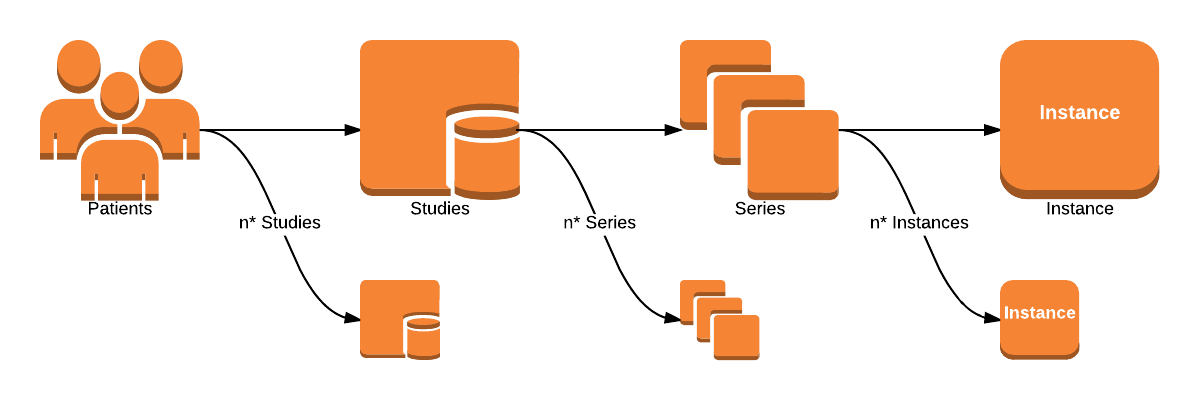
\includegraphics[width=\textwidth]{images/fig025}
\caption{[DOI: \href{https://doi.org/10.13140/RG.2.2.19014.32321}{10.13140/RG.2.2.19014.32321}] This illustrative diagram shows that a given patient benefits from a set of medical imaging studies. Each study is made from a set of series. Each series is, in turn, a set of instances.}
\label{fig:fig025}
\end{figure}
%%%%%%%%%%%%%%%%%%%%%%%%%%%%%%%%%%%%%%%%%%%%%%%%%%%

Within the \ac{DICOM} terminology, each element within the dataset is referred to as a \ac{DICOM} tag.
These tags serve as keys that uniquely identify and categorize different aspects of medical information.
To ensure consistency and standardization, there exists an official dictionary that normalizes the list of \ac{DICOM} tags.
Furthermore, to enhance the readability of \ac{DICOM} files, it is common practice to assign meaningful names to these tags.
For instance, tags such as \texttt{PatientName} and \texttt{StudyDescription} provide descriptive information about the patient and the study, respectively.

In the context of this thesis work, the \ac{DICOM} format and its associated technologies play a vital role in storing and managing the vast amount of data generated during medical imaging examinations.
Efficient storage, organization, and access to exams and patient information are made possible by leveraging the capabilities of \ac{DICOM}.
These functionalities are crucial for supporting the various stages of the radiological workflow, including examination, diagnosis, and reporting, ultimately contributing to improved patient care and outcomes.

\section{Exploring Medical Imaging Storage and Integration}
\label{sec:app001008}

This section provides a detailed exploration of medical imaging storage and integration, building upon the summary presented in Section~\ref{sec:chap002008} of Chapter~\ref{chap:chap002}.
Efficient storage and accessibility of medical images are crucial for streamlined workflows and accurate breast cancer diagnoses.
This section focuses on utilizing \ac{PACS} systems~\cite{carter2018digital}, which provide storage and user-friendly access to \ac{DICOM} images from different modalities (Figure~\ref{fig:fig113}).
Integrating specific packages and environments seamlessly enhances clinical setups with \ac{PACS} technologies.
Our platform offers comprehensive tools for multimodality strategies, facilitating interactive image visualization, manipulation, and study navigation within a web browser.
This integration simplifies multimodality deployment, improving breast cancer diagnosis efficiency.

%%%%%%%%%%%%%%%%%%%%%%%%%%%%%%%%%%%%%%%%%%%%%%%%%%%
\begin{figure}[ht]
\centering
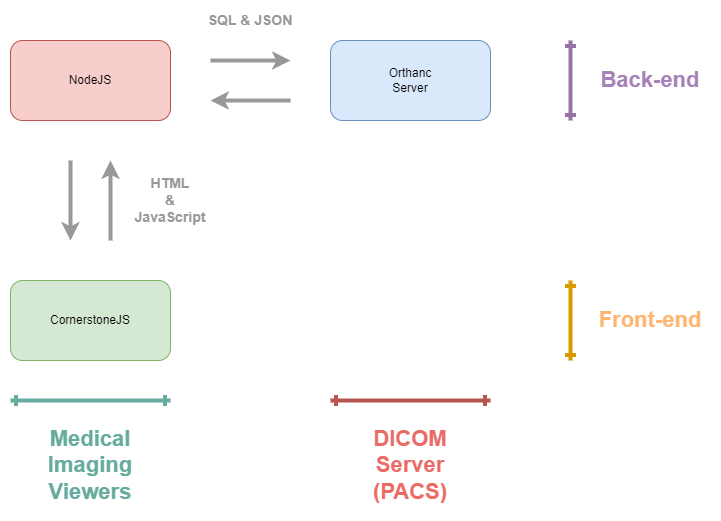
\includegraphics[width=0.85\textwidth]{images/fig113}
\caption{[DOI: \href{https://doi.org/10.13140/rg.2.2.13834.62405}{10.13140/RG.2.2.13834.62405}] Schematic demonstrating both {\bf Front-end} and {\bf Back-end} components of the system with integrated medical imaging solutions. In our solution, we show the use of technologies such as {\bf NodeJS} and {\bf CornerstoneJS} for the {\bf Medical Imaging Viewers}, as well as the {\bf Orthanc Server} for the {\bf DICOM Server (PACS)} component. The communication is via TCP.}
\label{fig:fig113}
\end{figure}
%%%%%%%%%%%%%%%%%%%%%%%%%%%%%%%%%%%%%%%%%%%%%%%%%%%

To enhance accessibility and collaboration, we have developed a web-based {\it framework} (Appendix~\ref{chap:app008}) that integrates a Front-end and Back-end ecosystem for efficient content management, image storage, and display~\cite{WO2022071818A1, 10.1145/3399715.3399744}.
Drawing inspiration from similar systems~\cite{HOSTETTER2018811}, our {\it framework} streamlines the handling of medical imaging data.
The Back-end architecture plays a crucial role in managing image storage and retrieval.
We utilized NodeJS (\href{https://nodejs.org/en}{nodejs.org}), a \acf{JS} framework (\href{https://www.w3schools.com/js/}{w3schools.com/js}), to create a cohesive Back-end that includes the web server, image storage, and content management.
With NodeJS, we achieved a robust and scalable platform for building fast network applications, particularly suited for data-intensive real-time applications across distributed devices.

NodeJS served as a WebSocket library for seamless server-client communication, enabling real-time, bidirectional data transmission for efficient delivery of medical images.
Using the net module of NodeJS, we established \ac{TCP} servers and clients to listen for incoming \ac{DICOM} or WebSocket connections~\cite{WO2022071818A1}.
Our web-based {\it framework} efficiently stores and retrieves medical image metadata using \ac{SQL} and \ac{JSON} databases, facilitating easy organization and retrieval of patient and exam information.
The \ac{JS}-based web server, powered by NodeJS, acts as the backbone of our Back-end implementation, facilitating data transmission between the \ac{DICOM} server and the web client.